\documentclass{beamer}
\usepackage[utf8]{inputenc}

\usetheme{Madrid}
\usecolortheme{default}
\usepackage{amsmath,amssymb,amsfonts,amsthm}
\usepackage{txfonts}
\usepackage{tkz-euclide}
\usepackage{listings}
\usepackage{adjustbox}
\usepackage{array}
\usepackage{tabularx}
\usepackage{gvv}
\usepackage{lmodern}
\usepackage{circuitikz}
\usepackage{tikz}
\usepackage{graphicx}
\usepackage{amsmath}

\setbeamertemplate{page number in head/foot}[totalframenumber]

\usepackage{tcolorbox}
\tcbuselibrary{minted,breakable,xparse,skins}



\definecolor{bg}{gray}{0.95}
\DeclareTCBListing{mintedbox}{O{}m!O{}}{%
  breakable=true,
  listing engine=minted,
  listing only,
  minted language=#2,
  minted style=default,
  minted options={%
    linenos,
    gobble=0,
    breaklines=true,
    breakafter=,,
    fontsize=\small,
    numbersep=8pt,
    #1},
  boxsep=0pt,
  left skip=0pt,
  right skip=0pt,
  left=25pt,
  right=0pt,
  top=3pt,
  bottom=3pt,
  arc=5pt,
  leftrule=0pt,
  rightrule=0pt,
  bottomrule=2pt,
  toprule=2pt,
  colback=bg,
  colframe=orange!70,
  enhanced,
  overlay={%
    \begin{tcbclipinterior}
    \fill[orange!20!white] (frame.south west) rectangle ([xshift=20pt]frame.north west);
    \end{tcbclipinterior}},
  #3,
}
\lstset{
    language=C,
    basicstyle=\ttfamily\small,
    keywordstyle=\color{blue},
    stringstyle=\color{orange},
    commentstyle=\color{green!60!black},
    numbers=left,
    numberstyle=\tiny\color{gray},
    breaklines=true,
    showstringspaces=false,
}


\title 
{4.4.17}
\date{September 10,2025}


\author 
{Abhiram Reddy-AI25BTECH11021}



\begin{document}


\frame{\titlepage}
%------------------------------------
\begin{frame}{Problem Statement}

A point \(\mathbf{P}\) divides the line segment joining the points \(\mathbf{A}(3, -5)\) and \(\mathbf{B}(-4, 8)\) such that 
\[
\frac{AP}{PB} = \frac{K}{1}.
\]
If \(\mathbf{P}\) lies on the line \(x + y = 0\), then find the value of \(K\).
\end{frame}

% Answer Step 1
\begin{frame}{Step 1: Represent points as vectors}
\[
\mathbf{A} = \begin{pmatrix} a_1 \\ a_2 \end{pmatrix}, \quad 
\mathbf{B} = \begin{pmatrix} b_1 \\ b_2 \end{pmatrix}.
\]
\end{frame}

\begin{frame}{Step 2: Section formula}
Since \(\mathbf{P}\) divides \(\mathbf{AB}\) in the ratio \(K : 1\),
\[
\mathbf{P} = \frac{K \mathbf{B} + \mathbf{A}}{K + 1}.
\]
\end{frame}

\begin{frame}{Step 3: Line equation condition}
Suppose the line is given as
\[
\mathbf{n}^\top \mathbf{x} = c, 
\quad \mathbf{n} = \begin{pmatrix} n_1 \\ n_2 \end{pmatrix}.
\]
Since \(\mathbf{P}\) lies on the line,
\[
\mathbf{n}^\top \mathbf{P} = c.
\]
\end{frame}

\begin{frame}{Step 4: Derive general formula for \(K\)}
\[
\mathbf{n}^\top (K\mathbf{B} + \mathbf{A}) = c(K+1),
\]
\[
K(\mathbf{n}^\top \mathbf{B} - c) = c - \mathbf{n}^\top \mathbf{A},
\]
\[
K = \frac{c - \mathbf{n}^\top \mathbf{A}}{\mathbf{n}^\top \mathbf{B} - c}.
\]
\end{frame}

\begin{frame}{Step 5: Substitute values}
Given
\[
\mathbf{A} = \begin{pmatrix} 3 \\ -5 \end{pmatrix}, \quad 
\mathbf{B} = \begin{pmatrix} -4 \\ 8 \end{pmatrix}, \quad 
\mathbf{n} = \begin{pmatrix} 1 \\ 1 \end{pmatrix}, \quad 
c = 0,
\]
\[
K = \frac{0 - (1\cdot 3 + 1\cdot (-5))}{(1\cdot (-4) + 1\cdot 8) - 0}
= \frac{2}{4}
= \frac{1}{2}.
\]
\end{frame}

\begin{frame}{Final Answer}
\[
\boxed{K = \tfrac{1}{2}}
\]
\end{frame}

% C code frame
\begin{frame}[fragile]
\frametitle{\textbf{C Code: Calculate Point P}}
\begin{lstlisting}[language=C]
#include <stdio.h>

void calculateP(double A[2], double B[2], double K, double P[2]) {
    P[0] = (K * B[0] + A[0]) / (K + 1);
    P[1] = (K * B[1] + A[1]) / (K + 1);
}

int main() {
    double A[2] = {3, -5};
    double B[2] = {-4, 8};
    double K = 0.5;  // example value for K
    double P[2];

    calculateP(A, B, K, P);

    printf("Coordinates of P are: (%.2f, %.2f)\n", P[0], P[1]);

    return 0;
}
\end{lstlisting}
\end{frame}

% Python Code frame 1
\begin{frame}[fragile]
\frametitle{\textbf{Python Plotting Code - Part 1}}
\begin{lstlisting}[language=Python]
import numpy as np
import matplotlib.pyplot as plt

# Given points A and B
A = np.array([3, -5])
B = np.array([-4, 8])

# Given ratio K
K = 0.5

# Calculate point P dividing AB in ratio K:1
P = (K * B + A) / (K + 1)
\end{lstlisting}
\end{frame}

% Python Code frame 2
\begin{frame}[fragile]
\frametitle{\textbf{Python Plotting Code - Part 2}}
\begin{lstlisting}[language=Python]
# Prepare line segment AB
line_AB_x = [A[0], B[0]]
line_AB_y = [A[1], B[1]]

# Prepare line x + y = 0 (y = -x)
x_vals = np.linspace(-10, 10, 400)
y_vals = -x_vals

# Plotting
plt.figure(figsize=(8, 8))
plt.plot(line_AB_x, line_AB_y, 'b-', label='Line segment AB')
plt.plot(x_vals, y_vals, 'g--', label='Line x + y = 0')
\end{lstlisting}
\end{frame}

% Python Code frame 3
\begin{frame}[fragile]
\frametitle{\textbf{Python Plotting Code - Part 3}}
\begin{lstlisting}[language=Python]
# Plot points
plt.plot(A[0], A[1], 'ro', label='Point A (3, -5)')
plt.plot(B[0], B[1], 'bo', label='Point B (-4, 8)')
plt.plot(P[0], P[1], 'mo', label=f'Point P (K={K})')

plt.xlabel('x')
plt.ylabel('y')
plt.title('Points A, B, P and line x + y = 0')
plt.legend()
plt.grid(True)
plt.axis('equal')

# Save plot
plt.savefig('python_plot.png')
plt.show()
\end{lstlisting}
\end{frame}




\begin{frame}{Plot}
    \centering
    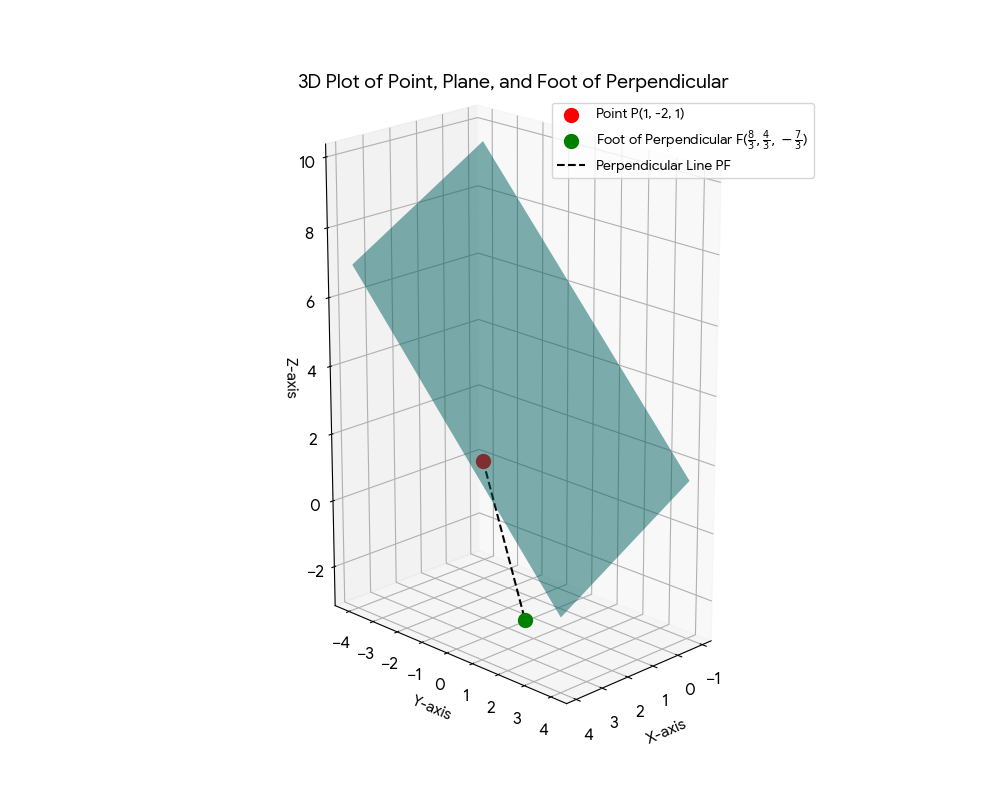
\includegraphics[width=\columnwidth, height=0.8\textheight, keepaspectratio]{figs/python_plot.png}     
\end{frame}


\end{document}